%%%%%%%%%%%%%%
%% Run LaTeX on this file several times to get Table of Contents,
%% cross-references, and citations.

%% If you have font problems, you may edit the w-bookps.sty file
%% to customize the font names to match those on your system.

%% w-bksamp.tex. Current Version: Feb 16, 2012
%%%%%%%%%%%%%%%%%%%%%%%%%%%%%%%%%%%%%%%%%%%%%%%%%%%%%%%%%%%%%%%%
%
%  Sample file for
%  Wiley Book Style, Design No.: SD 001B, 7x10
%  Wiley Book Style, Design No.: SD 004B, 6x9
%
%
%  Prepared by Amy Hendrickson, TeXnology Inc.
%  http://www.texnology.com
%%%%%%%%%%%%%%%%%%%%%%%%%%%%%%%%%%%%%%%%%%%%%%%%%%%%%%%%%%%%%%%%

%%%%%%%%%%%%%
% 7x10
%\documentclass{wileySev}

% 6x9
\documentclass{wileySix}

\usepackage{graphicx}
\usepackage{listings}

\usepackage{color}
 
\definecolor{codegreen}{rgb}{0,0.6,0}
\definecolor{codegray}{rgb}{0.5,0.5,0.5}
\definecolor{codepurple}{rgb}{0.58,0,0.82}
\definecolor{backcolour}{rgb}{0.95,0.95,0.92}
 
\lstdefinestyle{mystyle}{
    backgroundcolor=\color{backcolour},   
    commentstyle=\color{codegreen},
    keywordstyle=\color{magenta},
    numberstyle=\tiny\color{codegray},
    stringstyle=\color{codepurple},
    basicstyle=\footnotesize,
    breakatwhitespace=false,         
    breaklines=true,                 
    captionpos=b,                    
    keepspaces=true,                 
    numbers=left,                    
    numbersep=5pt,                  
    showspaces=false,                
    showstringspaces=false,
    showtabs=false,                  
    tabsize=2,
    language=sh
}
 
\lstset{style=mystyle}

%%%%%%%
%% for times math: However, this package disables bold math (!)
%% \mathbf{x} will still work, but you will not have bold math
%% in section heads or chapter titles. If you don't use math
%% in those environments, mathptmx might be a good choice.

% \usepackage{mathptmx}

% For PostScript text
\usepackage{w-bookps}

%%%%%%%%%%%%%%%%%%%%%%%%%%%%%%%%%%%%%%%%%%%%%%%%%%%%%%%%%%%%%%%%
%% Other packages you might want to use:

% for chapter bibliography made with BibTeX
% \usepackage{chapterbib}

% for multiple indices
% \usepackage{multind}

% for answers to problems
% \usepackage{answers}

%%%%%%%%%%%%%%%%%%%%%%%%%%%%%%
%% Change options here if you want:
%%
%% How many levels of section head would you like numbered?
%% 0= no section numbers, 1= section, 2= subsection, 3= subsubsection
%%==>>
\setcounter{secnumdepth}{3}

%% How many levels of section head would you like to appear in the
%% Table of Contents?
%% 0= chapter titles, 1= section titles, 2= subsection titles, 
%% 3= subsubsection titles.
%%==>>
\setcounter{tocdepth}{2}

%% Cropmarks? good for final page makeup
%% \docropmarks

%%%%%%%%%%%%%%%%%%%%%%%%%%%%%%
%
% DRAFT
%
% Uncomment to get double spacing between lines, current date and time
% printed at bottom of page.
% \draft
% (If you want to keep tables from becoming double spaced also uncomment
% this):
% \renewcommand{\arraystretch}{0.6}
%%%%%%%%%%%%%%%%%%%%%%%%%%%%%%

%%%%%%% Demo of section head containing sample macro:
%% To get a macro to expand correctly in a section head, with upper and
%% lower case math, put the definition and set the box 
%% before \begin{document}, so that when it appears in the 
%% table of contents it will also work:

\newcommand{\VT}[1]{\ensuremath{{V_{T#1}}}}

%% use a box to expand the macro before we put it into the section head:

\newbox\sectsavebox
\setbox\sectsavebox=\hbox{\boldmath\VT{xyz}}

%%%%%%%%%%%%%%%%% End Demo


\begin{document}


\booktitle{Cerdas Menguasai GIS}
\subtitle{Dalam 24 Jam}

\authors{Rolly M. Awangga\\
\affil{Informatics Research Center}
%Floyd J. Fowler, Jr.\\
%\affil{University of New Mexico}
}

\offprintinfo{Cerdas Menguasai Git, First Edition}{Rolly M. Awangga}

%% Can use \\ if title, and edition are too wide, ie,
%% \offprintinfo{Survey Methodology,\\ Second Edition}{Robert M. Groves}

%%%%%%%%%%%%%%%%%%%%%%%%%%%%%%
%% 
\halftitlepage

\titlepage


\begin{copyrightpage}{2019}
%Survey Methodology / Robert M. Groves . . . [et al.].
%\       p. cm.---(Wiley series in survey methodology)
%\    ``Wiley-Interscience."
%\    Includes bibliographical references and index.
%\    ISBN 0-471-48348-6 (pbk.)
%\    1. Surveys---Methodology.  2. Social 
%\  sciences---Research---Statistical methods.  I. Groves, Robert M.  II. %
%Series.\\
%
%HA31.2.S873 2007
%001.4'33---dc22                                             2004044064
\end{copyrightpage}

\dedication{`Jika Kamu tidak dapat menahan lelahnya belajar, 
Maka kamu harus sanggup menahan perihnya Kebodohan.'
~Imam Syafi'i~}

\begin{contributors}
\name{Rolly Maulana Awangga,} Informatics Research Center., Politeknik Pos Indonesia, Bandung,
Indonesia



\end{contributors}

\contentsinbrief
\tableofcontents
\listoffigures
\listoftables
\lstlistoflistings


\begin{foreword}
Sepatah kata dari Kaprodi, Kabag Kemahasiswaan dan Mahasiswa
\end{foreword}

\begin{preface}
Buku ini diciptakan bagi yang awam dengan git sekalipun.

\prefaceauthor{R. M. Awangga}
\where{Bandung, Jawa Barat\\
Februari, 2019}
\end{preface}


\begin{acknowledgments}
Terima kasih atas semua masukan dari para mahasiswa agar bisa membuat buku ini 
lebih baik dan lebih mudah dimengerti.

Terima kasih ini juga ditujukan khusus untuk team IRC yang 
telah fokus untuk belajar dan memahami bagaimana buku ini mendampingi proses 
Intership.
\authorinitials{R. M. A.}
\end{acknowledgments}

\begin{acronyms}
\acro{ACGIH}{American Conference of Governmental Industrial Hygienists}
\acro{AEC}{Atomic Energy Commission}
\acro{OSHA}{Occupational Health and Safety Commission}
\acro{SAMA}{Scientific Apparatus Makers Association}
\end{acronyms}

\begin{glossary}
\term{git}Merupakan manajemen sumber kode yang dibuat oleh linus torvald.

\term{bash}Merupakan bahasa sistem operasi berbasiskan *NIX.

\term{linux}Sistem operasi berbasis sumber kode terbuka yang dibuat oleh Linus Torvald
\end{glossary}

\begin{symbols}
\term{A}Amplitude

\term{\hbox{\&}}Propositional logic symbol 

\term{a}Filter Coefficient

\bigskip

\term{\mathcal{B}}Number of Beats
\end{symbols}

\begin{introduction}

%% optional, but if you want to list author:

\introauthor{Rolly Maulana Awangga, S.T., M.T.}
{Informatics Research Center\\
Bandung, Jawa Barat, Indonesia}

Pada era disruptif  \index{disruptif}\index{disruptif!modern} 
saat ini. git merupakan sebuah kebutuhan dalam sebuah organisasi pengembangan perangkat lunak.
Buku ini diharapkan bisa menjadi penghantar para programmer, analis, IT Operation dan Project Manajer.
Dalam melakukan implementasi git pada diri dan organisasinya.

Rumusnya cuman sebagai contoh aja biar keren\cite{awangga2018sampeu}.

\begin{equation}
ABC {\cal DEF} \alpha\beta\Gamma\Delta\sum^{abc}_{def}
\end{equation}

\end{introduction}

%%%%%%%%%%%%%%%%%%Isi Buku_


\chapter{PENGENALAN SISTEM INFORMASI GEOGRAFIS}
\section{Definisi GIS} 
Sistem Informasi Geografis atau disingkat SIG dalam bahasa Inggris Geographic Information System (disingkat GIS) merupakan sistem informasi khusus yang mengelola data yang memiliki informasi spasial (bereferensi keruangan). Atau dalam arti yang lebih sempit adalah sistem komputer yang memiliki kemampuan untuk membangun, menyimpan, mengelola dan menampilkan informasi bereferensi geografis atau data geospasial untuk mendukung pengambilan keputusan dalam perencanaan dan pengelolaan suatu wilayah, misalnya data yang diidentifikasi menurut lokasinya, dalam sebuah database. Para praktisi juga memasukkan orang yang membangun dan mengoperasikannya dan data sebagai bagian dari sistem ini. 
Teknologi Sistem Informasi Geografis dapat digunakan untuk investigasi ilmiah, pengelolaan sumber daya, perencanaan pembangunan, kartografi dan perencanaan rute. Misalnya, SIG bisa membantu perencana untuk secara cepat menghitung waktu tanggap darurat saat terjadi bencana alam, atau SIG dapat digunaan untuk mencari lahan basah (wetlands) yang membutuhkan perlindungan dari polusi atau dapat digunakan mencari informasi sebuah tempat khusus dan banyak manfaat lain yang dapat ikembangkan dalam sistem informasi geografis ini. 

\subsection{Pengertian GIS Menurut Para Ahli}
\begin{enumerate}

\item \textbf{Aronaff (1989)}
\subitem SIG adalah sistem informasi yang didasarkan pada kerja komputer yang memasukkan, mengelola, memanipulasi dan menganalisis data serta memberi uraian.

\item \textbf{Burrough (1986)}
\subitem SIG merupakan alat yang bermanfaat untuk pengumpulan, penimbunan, pengambilan kembali data yang diinginkan dan penayangan data keruangan yang berasal dari kenyataan dunia.

\item \textbf{Murai (1999)}
\subitem SIG sebagai sistem informasi yang digunakan untuk memasukkan, menyimpan, memanggil kembali, mengolah, menganalisis dan menghasilkan data bereferensi geografis atau data geospasial untuk mendukung pengambilan keputusan dalam perencanaan dan pengelolaan penggunaan lahan, sumber daya alam, lingkungan, transportasi, fasilitas kota, dan pelayanan umum lainnya.

\item \textbf{Marble et al (1983)}
\subitem SIG merupakan sistem penanganan data keruangan.  Bernhardsen (2002) SIG sebagai sistem komputer ang digunakan untuk memanipulasi data geografi. Sistem ini diimplementasikan dengan perangkat keras dan perangkat lunak komputer yang berfungsi untuk akusisi dan verifikasi data, kompilasi data, penyimpanan data, perubahan dan pembaharuan data, manajemen dan pertukaran data, manipulasi data, pemanggilan dan presentasi data serta analisa data.

\item \textbf{Gistut (1994)}
\subitem SIG adalah sistem yang dapat mendukung pengambilan keputusan spasial dan mampu mengintegrasikan deskripsi-deskripsi lokasi dengan karakteristik-karakteristik fenomena yang ditemukan di lokasi tersebut. SIG yang lengkap mencakup metodologi dan teknologi yang diperlukan, yaitu data spasial perangkat keras, perangkat lunak dan struktur organisasi  Berry (1988) SIG merupakan sistem informasi, referensi internal, serta otomatisasi data keruangan.

\item \textbf{Calkin dan Tomlison (1984)}
\subitem SIG merupakan sistem komputerisasi data yang penting.  Linden, (1987) SIG adalah sistem untuk pengelolaan, penyimpanan, pemrosesan (manipulasi), analisis dan penayangan data secara spasial terkait dengan muka bumi.

\item \textbf{Alter}
\subitem SIG adalah sistem informasi yang mendukung pengorganisasian data, sehingga dapat diakses dengan menunjuk daerah pada sebuah peta.

\item \textbf{Prahasta}
\subitem SIG merupakan sejenis software yang dapat digunakan untuk pemasukan, penyimpanan, manipulasi, menampilkan, dan keluaran informasi geografis berikut atribut-atributnya.  Petrus Paryono SIG adalah sistem berbasis komputer yang digunakan untuk menyimpan, manipulasi dan menganalisis informasi geografi. Dari definisi-definisi dari para ahli di atas dapat disimpulkan bahwa SIG merupakan pengelolaan data geografis yang didasarkan pada kerja komputer (mesin).

\item \textbf{Petrus Paryono}
\subitem SIG adalah sistem berbasis komputer yang digunakan untuk menyimpan, manipulasi dan menganalisis informasi geografi. Dari definisi-definisi dari para ahli di atas dapat disimpulkan bahwa SIG merupakan pengelolaan data geografis yang didasarkan pada kerja komputer (mesin).

\item \textbf{Chrisman (1997)}
\subitem SIG adalah sistem yang terdiri dari perangkat keras , perangkat lunak , data,manusia (brainware) organisasi dan lembaga yang digunakan untuk mengumpulkan,menyimpan,menganalisis dan menyebarkan informasi informasi mengenai daerah daerah di permukaan bumi.

\item \textbf{Lukman (1993)}
\subitem Menyatakan bahwa sistem informasi geografi menyajikan informasi keruangan beserta atributnya yang terdiri dari beberapa komponen utama yaitu:
\begin{enumerate}
\item Masukan data merupakan proses pemasukan data pada komputer dari peta (peta topografi dan peta tematik), data statistik, data hasil analisis penginderaan jauh data hasil pengolahan citra digital penginderaan jauh, dan lain-lain. Data-data spasial dan atribut baik dalam bentuk analog maupun data digital tersebut dikonversikan kedalam format yang diminta oleh perangkat lunak sehingga terbentuk basisdata (database).
\item Penyimpanan data dan pemanggilan kembali (data storage dan retrieval) ialah penyimpanan data pada komputer dan pemanggilan kembali dengan cepat (penampilan pada layar monitor dan dapat ditampilkan/cetak pada kertas).

\item Manipulasi data dan analisis ialah kegiatan yang dapat dilakukan berbagai macam perintah misalnya overlay antara dua tema peta, membuat buffer zone jarak tertentu dari suatu area atau titik dan sebagainya. Anon (2003) mengatakan bahwa manipulasi dan analisis data merupakan ciri utama dari SIG. Kemampuan SIG dalam melakukan analisis gabungan dari data spasial dan data atribut akan menghasilkan informasi yang berguna untuk berbagai aplikasi.

\item Pelaporan data ialah dapat menyajikan data dasar, data hasil pengolahan data dari model menjadi bentuk peta atau data tabular. Menurut Barus dan wiradisastra (2000) Bentuk produk suatu SIG dapat bervariasi baik dalam hal kualitas, keakuratan dan kemudahan pemakainya. Hasil ini dapat dibuat dalam bentuk peta-peta, tabel angka-angka: teks di atas kertas atau media lain (hard copy), atau dalam cetak lunak (seperti file elektronik).
\end{enumerate}

\item \textbf{Barus dan Wiradisastra (2000)} 
\subitem Mengungkapkan bahwa SIG adalah alat yang handal untuk menangani data spasial, dimana dalam SIG data dipelihara dalam bentuk digital sehingga data ini lebih padat dibanding dalam bentuk peta cetak, tabel atau dalam bentuk konvensional lainnya yang akhirnya akan mempercepat pekerjaan dan meringankan biaya yang diperlukan.
Sarana utama untuk penanganan data spasial adalah SIG. SIG didesain untuk menerima data spasial dalam jumlah besar dari berbagai sumber dan mengintergrasikannya menjadi sebuah informasi, salah satu jenis data ini adalah data pengindraan jauh. Pengindraan jauh mempunyai kemampuan menghasilkan data spasial yang susunan geometrinya mendekati keadaan sebenarnya dengan cepat dan dalam jumlah besar. 
SIG akan memberi nilai tambah pada kemampuan pengindraan jauh dalam menghasilkan data spasial yang besar dimana pemanfaatan data pengindraan jauh tersebut tergantung pada cara penanganan dan pengolahan data yang akan mengubahnya menjadi informasi yang berguna.

\item \textbf{Indrawati (2002)}
\subitem Aplikasi SIG dapat digunakan untuk berbagai kepentingan selama data yang diolah memiliki refrensi geografi, maksudnya data tersebut terdiri dari fenomena atau objek yang dapat disajikan dalam bentuk fisik serta memiliki lokasi keruangan.

\item \textbf{Dulbahri (1993)}
\subitem Tujuan pokok dari pemanfaatan Sistem Informasi Geografis adalah untuk mempermudah mendapatkan informasi yang telah diolah dan tersimpan sebagai atribut suatu lokasi atau obyek. Ciri utama data yang bisa dimanfaatkan dalam Sistem Informasi Geografis adalah data yang telah terikat dengan lokasi dan merupakan data dasar yang belum dispesifikasi.
\end{enumerate}

\section{Komponen Sistem Informasi Geografis}
Komponen-komponen pendukung SIG terdiri dari lima komponen yang bekerja secara terintegrasi yaitu perangkat keras (hardware), perangkat lunak (software), data, manusia, dan metode yang dapat diuraikan sebagai berikut:

\subsection{Perangkat Keras (Hardware)}
 Perangkat keras SIG adalah perangkat-perangkat fisik yang merupakan bagian dari sistem komputer yang mendukung analisis geografi dan pemetaan. Perangkat keras SIG mempunyai kemampuan untuk menyajikan citra dengan resolusi dan kecepatan yang tinggi serta mendukung operasi operasi basis data dengan volume data yang besar secara cepat. Perangkat keras SIG terdiri dari beberapa bagian untuk menginput data, mengolah data, dan mencetak hasil proses. Berikut ini pembagian berdasarkan proses :

\begin{enumerate}
\item CPU (unit pemroses utama). Perangkat ini merupakan bagian dari sistem komputer yang bertindak sebagai tempat untuk pemerosessan semua instruksi-instruksi dan program (processor). Selain itu, CPU juga berfungsi untuk mengendalikan seluruh operasi yang ada di dalam lingkungan sistem komputer yang bersangkutan. 

\item RAM. Perangkat ini digunakan oleh CPU untuk menyimpan (sementara) semua data dan program yang dimasukan melalui input device. Baik untuk jangka waktu yang panjang maupun pendek. Kebutuhan GIS mengenai RAM ini juga sangat bervariasi seperti halnya CPU di atas. 

\item Storage. Perangkat ini merupakan tempat penyimpanan data secara permanen atau semi permanen (temporary). Bila dibandingkan dengan RAM, akses pada media ini agak lambat. Harddisk,disket,CD-ROM,flash disk (yang terkoneksi melalui USB-port), dan pita magnetis merupakan contoh-contoh dari kelompok perangkat ini. Kebutuhan storage seperti ini sangat bervariasi mulai dari GIS yang satu ke GIS yang lain.

\item Input deivce. Perangkat ini merupakan peralatan-peralatan yang digunakan untuk memasukan data ke dalam perangkat GIS. Yang termasuk ke dalam perangkat ini adalah keyboard, mouse, digitaizer, scaner, kamera digital, dan sebagainya.

\item Output device. Perangkat ini merupakan peralatan-peralatan yang digunakan untuk merepresentasikan data dan atau informasi GIS. Yang termasuk ke dalam perangkat ini adalah layer monitor, printer plotter, dan sebagainya.

\item Peripheral (lainnya). Perangkat pelengkap ini merupaka bagian dari sistem komputer GIS yang belum termasuk ke dalam perangkat-perangkat yang telah di sebutkan di atas. Untuk GIS yang kecil dan sederhana peripheral kemungkinan sama sekali tidak diperlukan, tetapi untuk GIS yang besar apalagi menggunakan jaringan dan dapat di peresentasikan di jaringan internet (web), maka diperlukan kabel-kabel jaringan, modem, ISP, router, card jaringan/ ethernet, CPU khusus untuk clients dan server, dan sebagainya.
Pada saat ini GIS sudah dapat digunakan pada platform destkop, PC, laptop, workstation, dan multi-user host. Dengan demikian, fungsionalitas perangkat tidak terlalu terikat erat dengan karakteristik-karakteristik perangkat fisiknya. 

\end{enumerate}
\section{Komponen Sistem Informasi Geografis}
Komponen-komponen pendukung SIG terdiri dari lima komponen yang bekerja secara terintegrasi yaitu perangkat keras (hardware), perangkat lunak (software), data, manusia, dan metode yang dapat diuraikan sebagai berikut:

\subsection{Perangkat Keras (Hardware)}
 Perangkat keras SIG adalah perangkat-perangkat fisik yang merupakan bagian dari sistem komputer yang mendukung analisis geografi dan pemetaan. Perangkat keras SIG mempunyai kemampuan untuk menyajikan citra dengan resolusi dan kecepatan yang tinggi serta mendukung operasi operasi basis data dengan volume data yang besar secara cepat. Perangkat keras SIG terdiri dari beberapa bagian untuk menginput data, mengolah data, dan mencetak hasil proses. Berikut ini pembagian berdasarkan proses :

\begin{enumerate}
\item CPU (unit pemroses utama). Perangkat ini merupakan bagian dari sistem komputer yang bertindak sebagai tempat untuk pemerosessan semua instruksi-instruksi dan program (\textit{processor}). Selain itu, CPU juga berfungsi untuk mengendalikan seluruh operasi yang ada di dalam lingkungan sistem komputer yang bersangkutan.

\item RAM. Perangkat ini digunakan oleh CPU untuk menyimpan (sementara) semua data dan program yang dimasukan melalui \textit{input device}. Baik untuk jangka waktu yang panjang maupun pendek. Kebutuhan GIS mengenai RAM ini juga sangat bervariasi seperti halnya CPU di atas. 

\item Storage. Perangkat ini merupakan tempat penyimpanan data secara permanen atau semi permanen (\textit{temporary}). Bila dibandingkan dengan RAM, akses pada media ini agak lambat. Harddisk,disket,CD-ROM,flash disk (yang terkoneksi melalui USB-port), dan pita magnetis merupakan contoh-contoh dari kelompok perangkat ini. Kebutuhan storage seperti ini sangat bervariasi mulai dari GIS yang satu ke GIS yang lain.

\item Input deivce. Perangkat ini merupakan peralatan-peralatan yang digunakan untuk memasukan data ke dalam perangkat GIS. Yang termasuk ke dalam perangkat ini adalah \textit{keyboard, mouse, digitaizer, scaner,} kamera digital, dan sebagainya.

\item Output device. Perangkat ini merupakan peralatan-peralatan yang digunakan untuk merepresentasikan data dan atau informasi GIS. Yang termasuk ke dalam perangkat ini adalah layer monitor, printer plotter, dan sebagainya.

\item Peripheral (lainnya). Perangkat pelengkap ini merupaka bagian dari sistem komputer GIS yang belum termasuk ke dalam perangkat-perangkat yang telah di sebutkan di atas. Untuk GIS yang kecil dan sederhana peripheral kemungkinan sama sekali tidak diperlukan, tetapi untuk GIS yang besar apalagi menggunakan jaringan dan dapat di peresentasikan di jaringan internet (web), maka diperlukan kabel-kabel jaringan, modem, ISP, router, card jaringan/ ethernet, CPU khusus untuk \textit{clients} dan \textit{server}, dan sebagainya.
\end{enumerate}

\subsection{Perangkat Lunak (Software)}
Perangkat lunak digunakan untuk melakukan proses menyimpan, menganalisa, memvisualkan data-data baik data spasial maupun non-spasial. Pada sistem komputer modern, perangkat lunak yang digunakan biasanya tidak dapat berdiri sendiri, tetapi terdiri dari beberapa layer. Model layer ini terdiri dari perangkat lunak sistem operasi, program-program pendukung sistemsistem khusus (special system utilites), dan perangkat lunak aplikasi.Perangkat lunak yang harus terdapat dalam komponen software SIG adalah:
\begin{enumerate}
\item Alat untuk memasukkan dan memanipulasi data SIG
\item Data Base Management System (DBMS)
\end{enumerate}

Perangkat lunak khusus aplikasi GIS sering digunakan untuk menjalankan tugas-tugas GIS. Perangkat lunak tipe ini banyak tersedia dalam bentuk paketpaket perangkat lunak yang terkadang masing-masingnya terdiri dari multiprogram yang terintegrasi untuk mendukung kemampuan-kemampuan khusus untuk pemetaan dijital, manajemen, dan analisis data geografi. 

Pemilihan perangkat lunak GIS akan sangat bergantung pada sejumlah faktor, termasuk tujuan-tujuan penggunaan atau aplikasi, biaya pembelian dan pemeliharaan, kesiapan dan kemampuan personil-personil pengguna berserta agen perangkat lunak yang yang bersangkutan. 

\subsection{Data}
Pada prinsipnya terdapat dua jenis data untuk mendukung SIG yaitu :
\begin{enumerate}
\item Data Spasial
\subitem Data spasial adalah gambaran nyata suatu wilayah yang terdapat di permukaan bumi. Umumnya direpresentasikan berupa grafik, peta, gambar dengan format digital dan disimpan dalam bentuk koordinat x,y (vektor) atau dalam bentuk image (raster) yang memiliki nilai tertentu.
Sebagian besar data yang akan ditangani dalam SIG merupakan data spasial yang berorientasi geografis, memiliki sistem koordinat tertentu sebagai dasar referensinya dan mempunyai dua bagian penting yang membuatnya berbeda dari data lain, yaitu informasi lokasi (spasial) dan informasi deskriptif (attribute) yang dijelaskan berikut ini :

\begin{enumerate}
\item Informasi lokasi (spasial), berkaitan dengan suatu koordinat baik koordinat geografi (lintang dan bujur) dan koordinat XYZ, termasuk diantaranya informasi datum dan proyeksi.
\item Informasi deskriptif (atribut) atau informasi non spasial, suatu lokasi yang memiliki beberapa keterangan yang berkaitan dengannya, contohnya : jenis vegetasi, populasi, luasan, kode pos, dan sebagainya.
\end{enumerate}

Secara sederhana format dalam bahasa komputer berarti bentuk dan kode penyimpanan data yang berbeda antara file satu dengan lainnya. Dalam SIG, data spasial dapat direpresentasikan dalam dua format,yaitu:
\begin{enumerate}
\item Data Vektor
Data vektor merupakan bentuk bumi yang direpresentasikan ke dalam kumpulan garis, area (daerah yang dibatasi oleh garis yang berawal dan berakhir pada titik yang sama), titik dan nodes (merupakan titik perpotongan antara dua buah garis).Keuntungan utama dari format data vektor adalah ketepatan dalam merepresentasikan fitur titik, batasan dan garis lurus. Pada gambar \ref{data_vektor} merupakan tampilannya
\begin{figure}[ht]
\centering
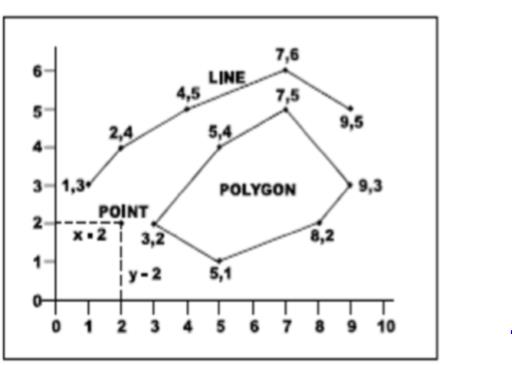
\includegraphics[width=0.5\textwidth]{pictures/data_vektor}
\caption{Data Vektor}
\label{data_vektor}
\end{figure}


\item Data Raster
Data raster (atau disebut juga dengan sel grid) adalah data yang dihasilkan dari sistem Penginderaan Jauh. Pada data raster,obyek geografis direpresentasikan sebagai struktur selgrid yang disebut dengan pixel(picture element). Pada gambar \ref{data_raster} merupakan tampilannya
\begin{figure}[ht]
\centering
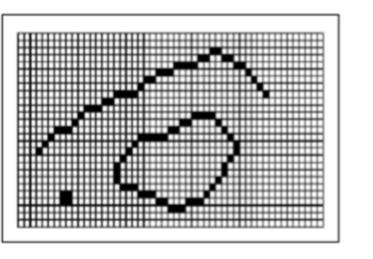
\includegraphics[width=0.5\textwidth]{pictures/data_raster}
\caption{Data Raster}
\label{data_raster}
\end{figure}
\end{enumerate}

\item Data Non Spasial (Atribut)
\subitem Data non spasial adalah data berbentuk tabel dimana tabel tersebut berisi informasi- informasi yang dimiliki oleh obyek dalam data spasial. Data tersebut berbentuk data tabular yang saling terintegrasi dengan data spasial yang ada.
Salah satu syarat SIG adalah data spasial, yang dapat diperoleh dari beberapa sumber antara lain:
\begin{enumerate}
\item Peta Analog
\subitem Peta analog (antara lain peta topografi, peta tanah dan sebagainya) yaitu peta dalam bentuk cetak. Pada umumnya peta analog dibuat dengan teknik kartografi, kemungkinan besar memiliki referensi spasial seperti koordinat, skala, arah mata angin dan sebagainya. Dalam tahapan SIG sebagai keperluan sumber data, peta analog dikonversi menjadi peta digital dengan cara format raster diubah menjadi format vektor melalui proses dijitasi sehingga dapat menunjukan koordinat sebenarnya dipermukaan bumi.

\item Data Sistem Penginderaan Jauh 
\subitem Penginderaan Jauh (antara lain citra satelit, foto udara dan sebagainya), merupakan sumber data yang terpenting bagi SIG karena ketersediaanya secara berkala dan mencakup area tertentu. Dengan adanya bermacam macam satelit di ruang angkasa dengan spesifikasinya masing masing, kita bisa memperoleh berbagai jenis citra satelit untuk beragam tujuan pemakaian. Data ini biasanya direpresentasikan dalam format raster.

\item Data Hasil Pengukuran Lapangan
\subitem  Data pengukuran lapangan yang dihasilkan berdasarkan teknik perhitungan tersendiri, pada umumnya data ini merupakan sumber data atribut contohnya: batas administrasi, batas kepemilikan lahan, batas persil, batas hak pengusahaan hutan dan lain - lain.

\item Data GPS (Global Positioning System)
\subitem Teknologi GPS memberikan terobosan penting dalam menyediakan data bagi SIG. Keakuratan pengukuran GPS semakin tinggi dengan berkembangnya teknologi. Data ini biasanya direpresentasikan dalam format vektor. 

\end{enumerate}
\end{enumerate}

\section{Ruang Lingkup Sistem Informasi Geografis}
Pada dasar nya sistem informasi geografis terdapat 6 proses yaitu:
\begin{enumerate}
\item Input data
\subitem Proses input data digunakan untuk menginputkan data spasial dan data non-spasial. Data spasial biasanya berupa peta analog. Untuk SIG harus menggunakan peta digital sehingga peta analog tersebut harus dikonversi ke dalam bentuk peta digital dengan menggunakan alat digitizer. Selain proses digitasi dapat juga dilakukan proses overlay dengan melakukan proses scanning pada peta analog.

\end{enumerate}




\chapter{TIPE TIPE DATA GEOPASIAL}
\section{TIPE TIPE DATA GEOPASIAL}
\begin{figure}[htbp]
		\centering
		\includegraphics[width=0.75\textwidth]{pictures/gis.jpg}
		\caption{Contoh gambar GIS}
		\label{labelgambar1}
		\end{figure}	
\subsection{Pembahasan}

Data Geospasial adalah data yang memuat lokasi geografis, dimensi atau ukuran, yang mana semua nya terdapat pada permukaan bumi. Data spasial SIG mempunyai dua bagian penting yang membuatnya berbeda dari data lain, yaitu informasi lokasi dan informasi atribut. Data spasial sistem informasi geografis yang berisi informasi lokasi (informasi spasial) contohnya adalah informasi lintang dan bujur, termasuk diantaranya informasi datum dan proyeksi.

Secara umum terdapat dua metode untuk menampilkan fitur geografis kedalam GIS  atau Sistem Informasi Geospasial. Pertama, dengan struktur data vektor (vector data strukture) yang terdiri dari sebuah gambaran titik geografis, baik yang berupa tanda titik, garis, maupun poligon. Model grafik vekor ini secara terpisah fitur geografis seperti batas  administratif, jalan, bangunan, dan sungai. Sebuah objek grafis biasanya terpisah fitur geografis biasanya dikaitkan dengan informasi yang mengandung penjelasan tentang atribut objek itu, dan informasi ini bisa saja disimpan di dalam berkas spreadsheets atau pangkalan data terpisah. Kedua, dengan struktur data raster (raster data strucuture), terdiri dari serangkaian sel atau pixels yang biasa dipakai untuk menggambarkan data gambar sebagai data yang berkisinambungan. Dalam struktur data yang demikian, ada unsur resolusi sebagai ukuran dari dimensi fitur geografis yang terwakili dalam bentuk pixel. Biasanya data raster ini dipakai untuk citra satelit, ortografi digital, model elevasi digital (digital elevation models, DEM), peta digital, dan sebagainya.

Contoh lain dari informasi spasial yang bisa digunakan untuk mengidentifikasikan lokasi misalnya adalah Kode Pos. Sedangkan Informasi Atribut (deskriptif) biasa disebut juga dengan informasi non-spasial. Suatu lokalitas bisa mempunyai beberapa atribut atau properti yang berkaitan dengannya; contohnya jenis vegetasi, populasi, pendapatan per tahun, dan lain-lain.\cite{prasetyo2018estimasi}Data geospasial dibagi mejadi dua tipe jenis, diantaranya:

\begin{enumerate}
\item Data vektor adalah data yang direpresentasikan sebagai suatu mosaik berupa garis (arc/\textit{line}), polygon (daerah yang dibatasi oleh garis yang berawal dan berakhir pada titik yang sama), titik/\textit{point} (node yang mempunyai label), dan \textit{nodes} (merupakan titik perpotongan antara dua buah garis). Keuntungan utama dari format data vektor adalah ketepatan dalam merepresentasikan fitur titik, batasan dan garis lurus. Kegunaan Data Vektor untuk analisa yang membutuhkan ketepatan posisi, misalnya pada basis data batas-batas kadaster. Contoh penggunaan lainnya adalah untuk mendefinisikan hubungan spasial dari beberapa fitur. Kelemahan data vektor yang utama adalah ketidakmampuannya dalam mengakomodasi perubahan gradual. Data vektor ini disimpan dalam file ber ekstensi .shp atau shapefile esri \cite{prasetyo2018estimasi}.
	\begin{enumerate}
	\item \textit{LINE}/\textit{PATH}
	\item \textit{POLYGON}
	\item \textit{POINT}
	\end{enumerate}
		\begin{figure}[htbp]
		\centering
		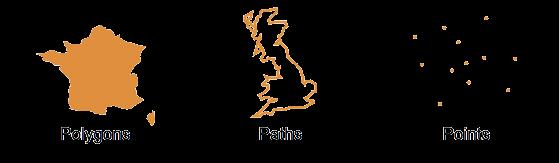
\includegraphics[width=0.75\textwidth]{pictures/datavektor.jpg}
		\caption{salah satu contoh gambar data vektor}
		\label{labelgambar2}
		\end{figure}	
	Pada gambar 1 terlihat 3 bentuk data jenis vector yaitu \textit{polygon} yang berbentuk wilayah, \textit{path} yang berbentuk garis dan point yang berbentuk titik titik.

		\begin{figure}[htbp]
		\centering
		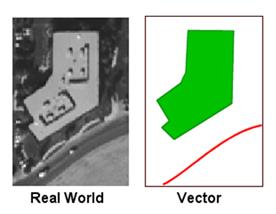
\includegraphics[width=0.65\textwidth]{pictures/olahdatavektor.jpg}
		\caption{perbandingan citra asli dengan hasil olah data vektor}
		\label{labelgambar3}
		\end{figure}
	Pada gambar 2 terlihat penerapan data \textit{vector polygon} dan \textit{ line} yang diterapkan pada salah satu bangunan. 
\item Data raster adalah data yang dihasilkan dari penginderaan jauh. Data Raster sering disebut juga dengan sel grid. Pada data raster, obyek geografis direpresentasikan sebagai struktur sel grid yang disebut dengan pixel (\textit{picture element}). Pada data raster, resolusi (definisi visual) tergantung pada ukuran pixel-nya. Dengan kata lain, resolusi pixel menggambarkan ukuran sebenarnya di permukaan bumi yang diwakili oleh setiap pixel pada citra.
Semakin kecil ukuran permukaan bumi yang direpresentasikan oleh satu sel, semakin tinggi resolusinya. Data raster sangat baik untuk merepresentasikan batas-batas yang berubah secara gradual, seperti jenis tanah, kelembaban tanah, vegetasi, suhu tanah, dan sebagainya. Kelemahan utama dari data raster adalah besarnya ukuran file; semakin tinggi resolusi grid-nya semakin besar pula ukuran filenya\cite{prasetyo2018estimasi}.
\end{enumerate}

Contoh data rester diantaranya:
\begin{enumerate}
\item Gambar citra satelit
\item Gambar PNG
\item Gambar JPG
\item Gambar Bitmap
\end{enumerate}
		\begin{figure}[htbp]
		\centering
		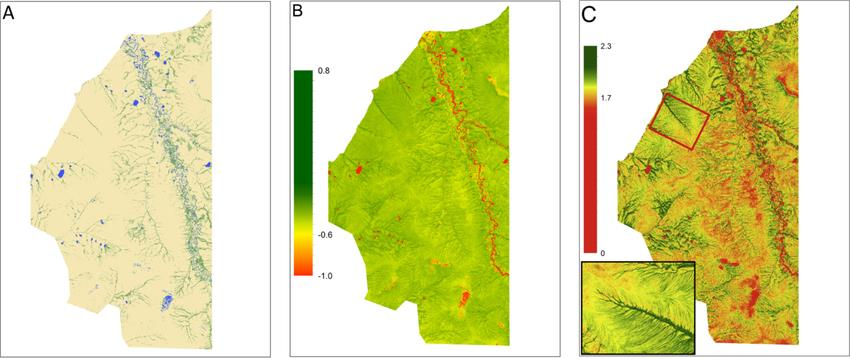
\includegraphics[width=0.65\textwidth]{pictures/dataraster.jpg}
		\caption{Gambar data raster dari tampak jauh menjadi gambar permukaan bumi seperti biasa}
		\label{labelgambar4}
		\end{figure}
Jika diliat dari penginderaan jarak jauh, maka data raster ini seperti gambar permukaan bumi pada biasanya, namun jika di \textit{zoom} lebih dekat maka akan muncul terlihat \textit{pixel pixel} nya.
		\begin{figure}[htbp]
		\centering
		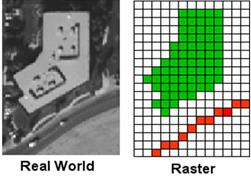
\includegraphics[width=0.65\textwidth]{pictures/datarasterzoom.jpg}
		\caption{Data raster jika di \textit{zoom} ke ukuran aslinya maka nampak \textit{pixel pixel} nya}
		\label{labelgambar5}
		\end{figure}
Pada gambar 4 terlihat penerapan data raster pada salah satu bangunan yang hasilnya berbentuk \textit{pixel pixel} gambar. \textit{Pixel} gambar tersebut muncul karna gambar telah di \textit{zoom} atau dalam bentuk resolusi yang kecil.

Berikut ditampilkan perbedaan nampak dari kedua data yang telah dipaparkan
		\begin{figure}[htbp]
		\centering
		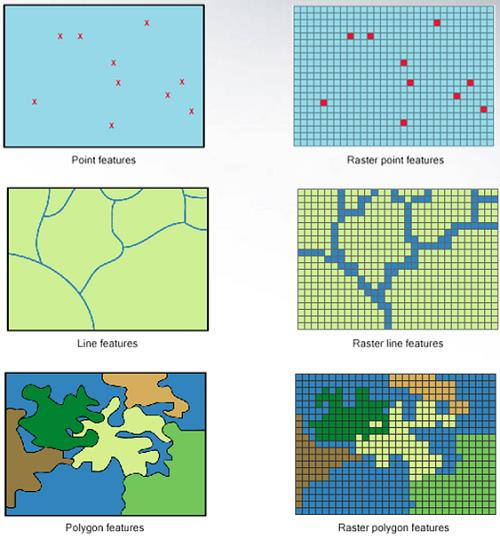
\includegraphics[width=0.65\textwidth]{pictures/perbedaan.jpg}
		\caption{Perbedaan data \textit{raster} dan \textit{vektor} pada 3 jenis penerapan.}
		\label{labelgambar6}
		\end{figure}
\section{Srukture Data GIS}
Data geografi meliputi informasi tentang posisi, hubungan topologi dan aspek spasial dari pemrosesan data. Data ini menggambarkan obyek dan fenomena geografinya. Obyek mengacu pada lokasinya pada permukaan bumi dengan menggunakan sistem koordinat 9dapat berupa lokal, nasional, maupun internasional). Sedangkan fenomena geografi dapat berupa konsep fenomenologi, sepertikota, sungai, dataran rendah/tinggi, bentuk serta struktur tanah, dan sebagainya. Fenomena geografi ini akan membawa ke dalam bentuk blok klasifikasi atau taksonomi secara hirarkis, seperti negara-propinsi-kabupaten-kecamatan-kelurahan, klasifikasi bentuk struktur tanah,vegetasi, dan sebagainya.Semua data geografi dapat disajikan dalam tiga bentuk dasar konsep topologi, yaitu:
\begin{enumerate}
\item Titik (point)
\item Garis (line)
\item Luasan(area)
\end{enumerate}
Setiap fenomena geografi pada dasarnya dapat disajikan ke dalam tiga bentuk dasar di atas, disertai dengan label yang menerangkan apa disajikan tersebut. Dalam aktivitas penelitian, perencanaan, atau pengambilan keputusan diperlukan data dan informasi yang baik dan teratur agar pekerjaan yang dilakukan dengan cepat dan tepat dapat diselesaikan. Pengaturan dan pengumpulan data secara manual biasa dilakukan berdasarkan hirarki topologi. Peta yang memuat berbagai macam data dan informasi, menyimpan data dalam bentuk topologi. Data keruangan dalam terminologi fisikal dan lokasi geografi. Bentuk data yang dapat dijadikan masukan kedalam notasi yang menunjukkan lokasi keruangan adalah titik, garis, dan area atau poligon. Semua data dari kenampakan, dan fenomena geografi dapat digambarkan melalui salah satu bentuk notasi tersebut.
\subsection{Cara Kerja Gis}
 GIS dapat mempersentasikan suatu model “real world” (dunia nyata) di atas layer monitor komputer sebagaimana lembaran-lembaran peta dapat mempresentasikan dunia nyata di atas kertas. Walaupun demikian, GIS memiliki kekuatan lebih dan daya flesksibelitas dari pada lembaran-lembaran peta kertas. Peta merupakan salah satu bentuk reperesentasi grafis miliki dunia nyata objekobjek yang direpresentasikan di atas peta disebut sebagai unsur-unsur peta atau map feature (sebagai contoh adalah sungai, jalan, gunung, bangunan, dan lainlain) karena peta mengorganisasikan unsur-unsurnya berdasarkan lokasi masingmasin, maka peta sangat baik di dalam memperlihatkan hubungan atau relasi yang dimiliki oleh unsur-unsurnya. Sebagai ilustrasi, berikut adalah contoh-contoh hubungan tersebut :
\begin{enumerate}
\item Suatu gedung terletak di dalam wilayah kecamatan tertentu.
\item Jembatan melintas di atas suatu sungai.
\item Bangunan kuno bersebelahan dengan taman.
\end{enumerate}
Berikut merupakan contoh peta kota bandung seperti pada gambar \ref{kotapetabandung}
\begin{figure}[ht]
	\centerline{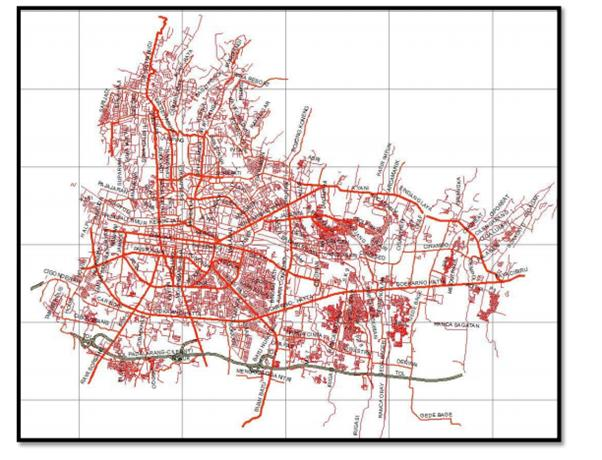
\includegraphics[width=0.60\textwidth]{pictures/bnd.jpg}}
	\caption{contoh peta kota bandung}
	\label{kotapetabandung}
	\end{figure}

\section{PENGENALAN TENTANG LONGITUDE,LATITUDE,BUJUR,DAN LINTANG}
\subsection{Sistem Koordinat}
Sistem koordinat dimaksudkan untuk memberikan peng-alamat-an terhadap setiap lokasi di permukaan bumi. Peng-alamat-an dengan sistem koordinat didasarkan atas jarak timur-barat dan utara-selatan suatu tempat dari suatu \textit{titik pangkal} tertentu. Jarak diukur dalam satuan derajat sudut yang dibentuk dari titik pangkal ke posisi tersebut yang melalui pusat bumi. Sedangkan titik pangkal ditetapkan berada di perpotongan belahan utara-selatan bumi (garis khatulistiwa) dengan garis yang membelah bumi timur-barat melalui kota Greenwich di Inggris. berikut adalah contoh gambar sistem kordinat dengan globe \ref{kordinat}
\begin{figure}[ht]
	\centerline{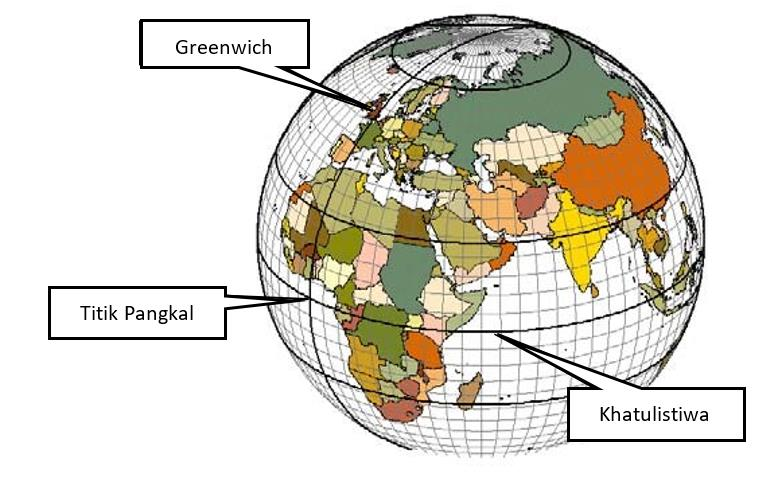
\includegraphics[width=0.70\textwidth]{pictures/kordinat.jpg}}
	\caption{contoh sitem koordinat dengan globe}
	\label{kordinat}
	\end{figure}

Posisi suatu tempat di-alamatkan dengan nilai koordinat garis bujur (longitude) dan lintang (latitude) yang melalui tempat itu. Garis bujur (longitude), sering juga disebut meridian, yaitu merupakan garis lurus yang menghubungkan kutub utara dan selatan bumi. Nilai koordinat garis bujur dimulai dari bujur 0 (drajat) yaitu di Greenwich, kemudian membesar ke arah timur dan barat sampai bertemu kembali di Garis batas tanggal internasional yaitu terletak di Selat Bering dengan nilai 180 (drajat). Garis bujur 0(drajat) sering sekali disebut prime meridian atau meridian Greenwich. Garis bujur ke arah barat diberi nilai negatif dan disebut dengan bujur barat (west longitude) serta disingkat BB. Sedangkan garis bujur yang ke arah timur diberi nilai positif dan disebut dengan bujur timur (east longitude) disingkat BT. Nilai koordinatnya didasarkan atas besarnya sudut yang terbentuk dari bujur 0 ke garis bujur tersebut melalui pusat bumi.

Untuk nilai koordinat lintang dimulai dari garis lingkaran katulistiwa yang diberi nilai 0(drajat). Selanjutnya garis lintang yang lain berupa lingkaran-lingkaran paralel (sejajar) khatulistiwa berada di sebelah utara dan selatan khatulistiwa. Lingkaran paralel di selatan disebut dengan garis lintang selatan (LS) dan diberi nilai negatif, sedangkan lingkaran paralel di utara diberi nilai positif  dan disebut garis lintang utara (LU). Nilai maksimum untuk koordinat garis lintang adalah 90(drajat) yaitu terletak di kutub-kutub bumi.

Lingkaran paralel yang merupakan representasi dari garis lintang ini semakin mengecil ukurannya dengan semakin jauh dari khatulistiwa. Sehingga jarak 1o timur-barat di khatulistiwa jauh lebih besar daripada jarak 1(derajat) timur-barat di tempat yang jauh dari khatulistiwa. Di khatulistiwa 1(derajat) timur-barat sama dengan 111,321 Km, tetapi di dekat kutub 1(derajat) timur-barat hanya beberapa meter saja. Itu sebabnya grid yang dibuat dari garis lintang dan garis bujur tampak berupa bujur sangkar di khatulistiwa dan berupa persegi panjang di daerah dekat kutub. Koordinat yaitu bilangan yang dipakai untuk menunjukkan lokasi suatu titik di garis permukaan atau ruang. Koordinat dapat memudahkan kita dalam menemukan letak suatu benda.
\subsection{Macam-macam Sistem Koordinat}
Adapun beberapa macam sistem koordinat, antara lain:
\begin{enumerate}
\item Sistem Koordinat Kartesius
Untuk menyatakan posisi sebuah benda dibutuhkan suatu sistem koordinat yang memiliki pusat koordinat dan sumbu koordinat. Sistem koordinat yang paling dasar/sederhana adalah sistem koordinat kartesius. Jika berbicara ruang dua dimensi, maka koordinat kartesius dua dimensi memiliki pusat di O dan dua sumbu koordinat yang saling tegak lurus yaitu x dan y. Dalam gambar dibawah ini, titik P dinyatakan dalam koordinat x dan y.
\end{enumerate}

\chapter{Membuat Data Vektor}


\section{Membuat Data Vektor}
Disusun oleh:

Eko cahyono putro 1164035
Nur Arkhamia Batubara 1164049

\subsection {Pengertian Data Vektor}
Data vektor merupakan tipe data yang umum ditemukan dalam SIG. Sebuah vektor pada intinya merupakan sesuatu yang berbentuk sebuah titik, atau garis yang menghubungkan titik-titik tersebut. Dengan kata lain, titik, garis, dan poligon merupakan vektor (garis lengkung merupakan vektor juga).

Salah satu hal yang penting untuk dicatat adalah \textit{layer} QGIS hanya mengandung satu tipe fitur. Artinya, satu layer tidak dapat mengandung fitur titik dan fitur garis, karena mereka merupakan tipe data yang berbeda. Namun apabila anda ingin memiliki sebuah \textit{file} yang memiliki \textit{polygon} sekolah dan file lain yang memiliki titik-titik sekolah, anda dapat menambahkan mereka sebagai dua \textit{layer} yang terpisah\cite{setiawan2018membuka}.

\subsection{Tutorial Membuat data vektor}
Hal pertama yang harus dilakukan untuk membuat data vektor adalah :
\begin{enumerate}
\item Menginstall python 3.6.6

\begin{figure}[htbp]
\centering
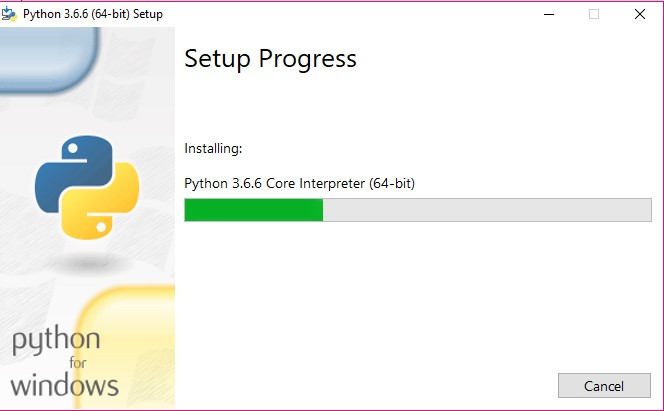
\includegraphics[width=0.75\textwidth]{pictures/python.jpg}
\caption{peroses instalasi \textit{python}}
\label{labelgambar1}
\end{figure}

\item Untuk mengecek apakan python sudah terinstall atau belum bisa menggunakan \textit{command prompt} pada computer anda.

\begin{figure}[htbp]
\centering
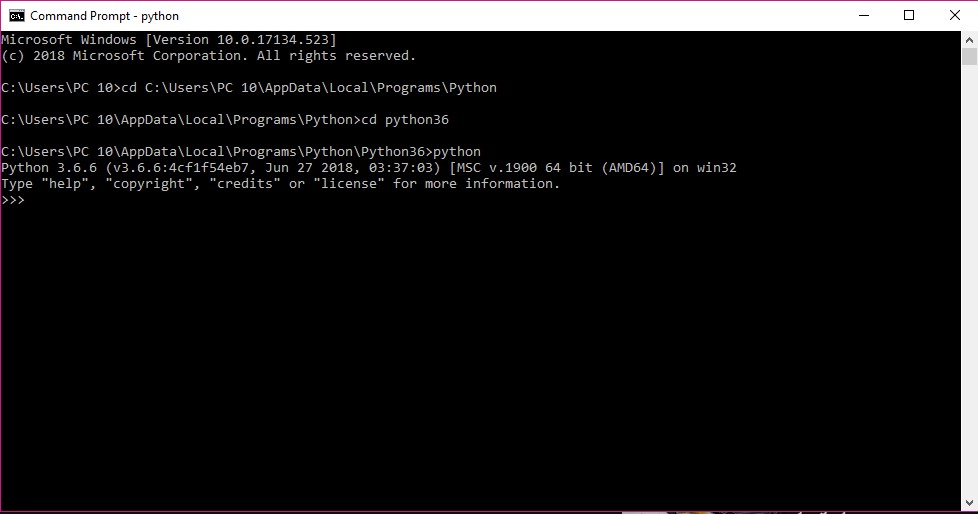
\includegraphics[width=0.75\textwidth]{pictures/pengecekanpython.jpg}
\caption{pengecekan \textit{python}}
\label{labelgambar2}
\end{figure}

Jika sudah muncul tampilan seperti digambar 1.2  ini maka python sudah terinstall.
\item Menginstall pyshp
\end{enumerate}

\begin{figure}[htbp]
\centering
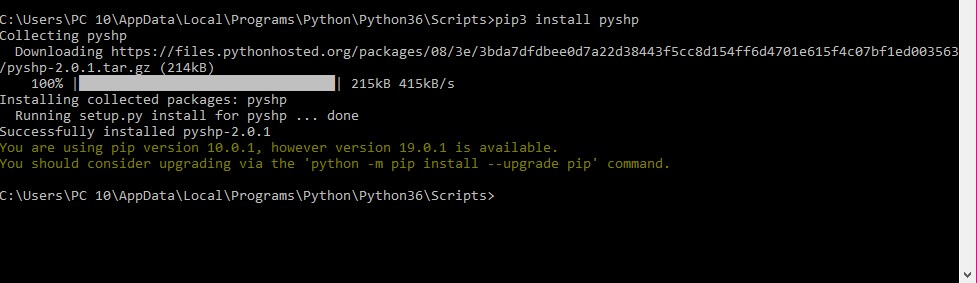
\includegraphics[width=1\textwidth]{pictures/installpy.jpg}
\caption{Mengintall Modul pyshp}
\label{labelgambar3}
\end{figure}
Kemudian menginstal modul pyshp dengan mengetik pip install pyshp di cmd. pyshp ini penting karena akan menggunakan modul ini untuk membuat data vector.Berikut langkah-langkah untuk membuat data vector yaitu beberapa bangun datar mulai dari point, polyline dan polygon. 

\subsection{Point}
Point adalah perintah untuk membuat sebuah titik. Adapun default-nya bentuk titik adalah noktah, akan tetapi bentuk tersebut bisa diubah sesuai dengan keinginan.

\begin{enumerate}
\item Untuk membuat file shp bisa menggunakan tools editor seperti notepad++, visualcode, sublime dan lain-lain, di sini saya menggunakan editor notepa+d+.  Buat script seperti gambar dibawah dan simpan dalam bentuk file .py:
\begin{figure}[htbp]
\centering
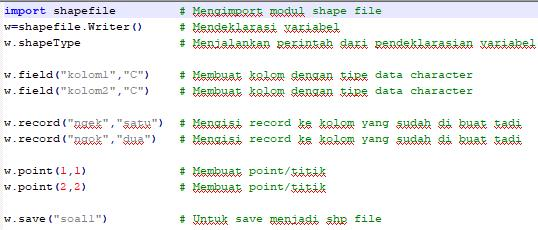
\includegraphics[width=1\textwidth]{pictures/soal1.jpg}
\caption{File Soal 1.py}
\label{labelgambar4}
\end{figure}

\item Jalankan program tersebut menggunakan \textit{command prompt}

\begin{figure}[htbp]
\centering
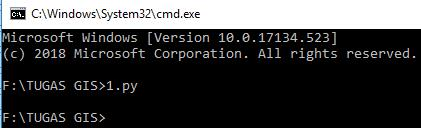
\includegraphics[width=1\textwidth]{pictures/pengujiansoal1.jpg}
\caption{Pengujian Soal1}
\label{labelgambar5}
\end{figure}
\end{enumerate}

\subsection{Tipe Data Geospasial}
Vektor dan data raster dua jenis data utama yang dipakai dalam Sistem Informasi Geospasial. Kedua vektor dan data raster mempunyai sistem referensi spasial. Ini adalah lintang dan bujur yang menentukan posisi di Bumi. Kita tahu ada dua model-model, yaitu data utama spasial vektor dan raster data. Tapi apa perbedaan antara raster dan vektor data? Kapan sebaiknya data ditampilkan sebagai raster atau vektor?
\begin{enumerate}
\item Vektor data tidak terdiri dari grid piksel. Sebaliknya, grafik vektor terdiri dari simpul dan jalur. Tiga jenis simbol dasar untuk data-data vektor adalah titik, garis dan poligon (untuk area). Sejak waktu subuh, peta tekah menggunakan simbol untuk mewakili fitur dunia nyata. Dalam terminologi Sistem Informasi Geospasial, fitur dunia nyata disebut dengan entitas spasial. 
Kegunaan Data Vektor Spatial Data Types adalah untuk menganalisa yang membutuhkan ketepatan posisi, misalnya pada basis data batas-batas kadaster: Contoh penggunaan lainnya adalah untuk mendefiniskan hubungan spasial dari beberapa fitur. Kelemahan data vektor yang utama adalah ketikmampuannya dalam mengakomodasi perubahan gradual. 

\end{enumerate}


\section{MEMBACA DATA VECTOR}
Data vector merupakan tipe data yang umum ditemukaaan dalam system informasi geografis. Sebuah vector pada inti merupakan sesuatu yang berbentuk sebuah titik, garis yang menghubungkan titik-titik tersebut.
Berikut langkah-langkah membaca data vector :
\begin{enumerate}
\item 1.py, buat script python berikut
\begin{lstlisting}
 import shapefile         
w=shapefile.Writer()
w.shapeType                 	
w.field("kolom1","C")
w.field("kolom2","C")
w.record("lidwina","satu")
w.record("riki","dua")
w.point(1,1)                  	  
w.point(2,2)
w.save("soal1")
\end{lstlisting}
\end{enumerate}

\chapter{SUMBER-SUMBER DATA GEOSPASIAL}
\section{SUMBER-SUMBER DATA GEOSPASIAL}

Dalam dunia geospasial tidak jauh dengan data spasial. Data spasial ibarat hokum mutlak diperlukan dalam membuat peta atau melakukan analisis spasial. Namun kendalanya tidak semua data-data yang diperlukan tersedia. Dalam uraian berikut akan membahas sumber data spasial dari open geodata.
\begin{enumerate}
\item \textbf{Ina Geoportal}
\subitem Ina Geoportal adalah sumber data geospasial resmi untuk Indonesia yang  dibangun, dipelihara dan diawasi langsung oleh Badan Informasi Geospasial (BIG) yang di mana merupakan lembaga pemerintah yang bertanggung jawab penuh atas data geospasial nasional. Melalui Ina Geoportal ini kita dapat men-download data-data peta rupa bumi dalam skala 250 ribu, 50 ribu dan 25 ribu. Proses mendapatkan datanya pun cukup mudah, Kita hanya perlu mengisikan Nama, email, jenis data RBI, jenis pengguna dan terakhir tentu saja kita harus menyetujui ketentuan undang-undang yang berlaku. Pada gambar \ref{labelgambar1} merupakan tampilannya  
\begin{figure}[ht]
\centering
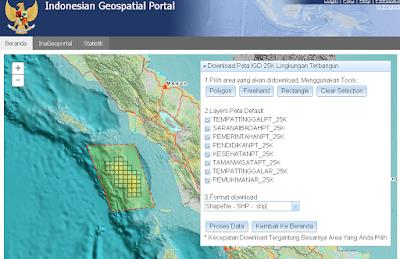
\includegraphics[width=0.5\textwidth]{pictures/ina_geospasial}
\caption{Ina Geoportal}
\label{labelgambar1}
\end{figure}

\item \textbf{USGS Earth Explorer}
\subitem USGS earth explorer merupakan sumber data spasial yang disediakan oleh lembaga survey geologi Amerika Serikat. Di earth explorer ini disediakan cukup banyak sekali data dengan berbagai macam tema, resolusi dan sensor, seperti citra satelit, Lidar, cuaca, radar, landcover dan lain sebagainya. Data-data tersedia umumnya mencakup data di wilayah Amerika. Namun, tidak hanya data-data tersebut yang tersedia melainkan data-data dengan cakupan global seperti data Digital Elevation Model (DEM), SRTM, citra satelit Landsat, monitoring vegetasi dan lain-lain.  Pada gambar \ref{labelgambar2} merupakan tampilannya  
\begin{figure}[ht]
\centering
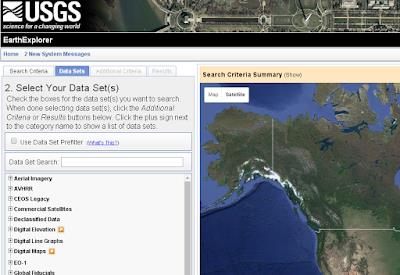
\includegraphics[width=0.5\textwidth]{pictures/usgs_earth_explorer}
\caption{USGS Earth Explorer}
\label{labelgambar2}
\end{figure}

\item \textbf{Worldclim}
\subitem Worldclim adalam sumber data geospasial yang menyediakan data curah hujan guna melakukan proses analisis spasial yang tersedia dalam format spasial. Worldclim menyuguhkan data curah hujan dan data iklim secara umum yang meliputi temperatur tahunan serta bulanan. Data ini diperoleh dari stasiun-stasiun cuaca di seluruh dunia yang dikumpulkan jadi satu dari tahun 1960-1990 (versi 1.4) dan 1970-2000 (versi 2). Data-data yang dikumpulkan kemudian diolah dan dianalisa sehingga dapat diprediksi data iklim untuk masa lalu, sekarang dan masa yang akan datang. Jadi, data ini bukan termasuk data realtime, akan tetapi analisa data iklim selama 30 tahun. Data wordclim dapat diperoleh dalam format raster dengan resolusi 1 km.  Pada gambar \ref{labelgambar3} merupakan tampilannya  

\begin{figure}[ht]
\centering
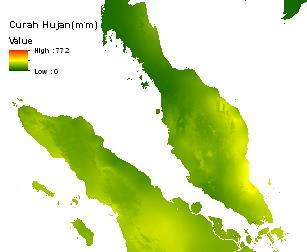
\includegraphics[width=0.5\textwidth]{pictures/data_worldclim}
\caption{USGS Data Worldclim}
\label{labelgambar3}
\end{figure}

\item \textbf{Global Forest Change}
\subitem Global Forest Change seperti merupakan data yang memonitor perubahan hutan. Data ini diperoleh dari analisis time series citra satelit Landsat mulai tahun 2000, dan terus diperbaharui secara berkala.  Sampai saat tulisan ini ditulis data yang tersedia sampai tahun 2014. Karena dianalisa dari data citra satelit Landsat maka data ini memiliki resolusi 30 meter, sehingga cocok untuk digunakan untuk analisa data dengan skala menengah. Data ini dikelola oleh Universitas Maryland Amerika Serikat. Cakupan data ini bersifat global dan dapat didownload dalam format “tif” dengan satu tile/scene berukuran 10 derajat x 10 derajat. Pada gambar \ref{labelgambar4} merupakan tampilannya
\begin{figure}[ht]
\centering
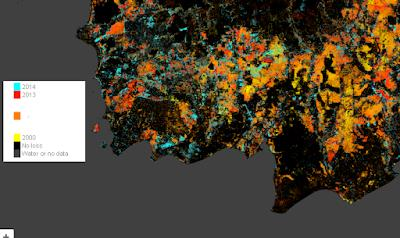
\includegraphics[width=0.5\textwidth]{pictures/Global_Forest_Change}
\caption{Global Forest Change}
\label{labelgambar4}
\end{figure}

\item \textbf{Soil Grid}
\subitem Soil Grid menyediakan informasi data tanah secara global. Karena sifatnya global tentu saja memiliki akurasi yang kasar dibandingkan dengan data jenis tanah dengan cakupan nasional atau provinsi. Data soil grid diperoleh dari analisa data-data tanah secara global yang diolah secara statisitk dengan metode kovarian dan regresi. Jenis tanah, kandungan carbon, air, gypsum dan lain-lain baik untuk tanah lapisan atas(top soil) maupun lapisan bawah (sub soil) adalah informasi yang dapat diperoleh dari Soil Grid. Data tersebut dapat didownload dalam format geotiff.  Pada gambar \ref{labelgambar5} merupakan tampilannya  

\begin{figure}[ht]
\centering
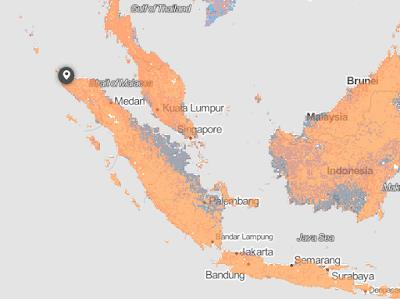
\includegraphics[width=0.5\textwidth]{pictures/Data_Tanah_Soil_Grid}
\caption{Data Tanah Soil Grid}
\label{labelgambar5}
\end{figure}

\item \textbf{USGS GloVis}
\subitem Sumber data geospasial yang menyediakan data geografis tentang bahaya alam yang mengancam kehidupan dan mata pencaharian, air, energi, mineral, dan sumber daya alam lainnya. Juga dampak kesehatan ekosistem dan lingkungan sekitar serta dampak perubahan iklim dan penggunaan lahan. Ilmuwan USGS GloVis sedang mengembangkan metode dan alat baru untuk memungkinkan informasi yang tepat waktu, relevan, dan berguna tentang Bumi dan prosesnya.  Pada gambar \ref{labelgambar6} merupakan tampilannya  

\begin{figure}[ht]
\centering
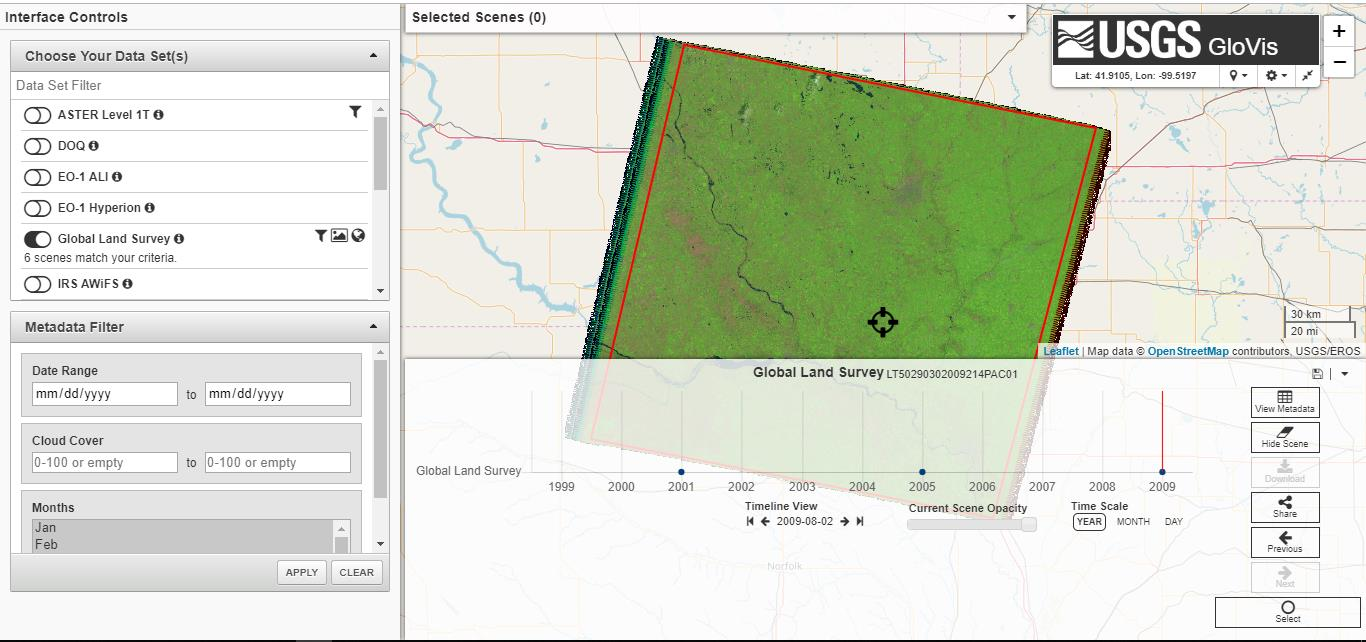
\includegraphics[width=0.5\textwidth]{pictures/USGS_GloVis}
\caption{USGS GloVis}
\label{labelgambar6}
\end{figure}

\item \textbf{Theia- Land Data Center}
\subitem Theia-Land Data Center adalah organisasi antar-lembaga nasional Prancis yang dirancang untuk mendorong penggunaan gambar yang didapatkan dari hasil pengamatan ruang permukaan tanah. Theia menawarkan komunitas ilmiah dan aktor kebijakan publik dari berbagai gambar di berbagai skala, metode dan layanan.  Pada gambar \ref{labelgambar7} merupakan tampilannya  
\begin{figure}[ht]
\centering
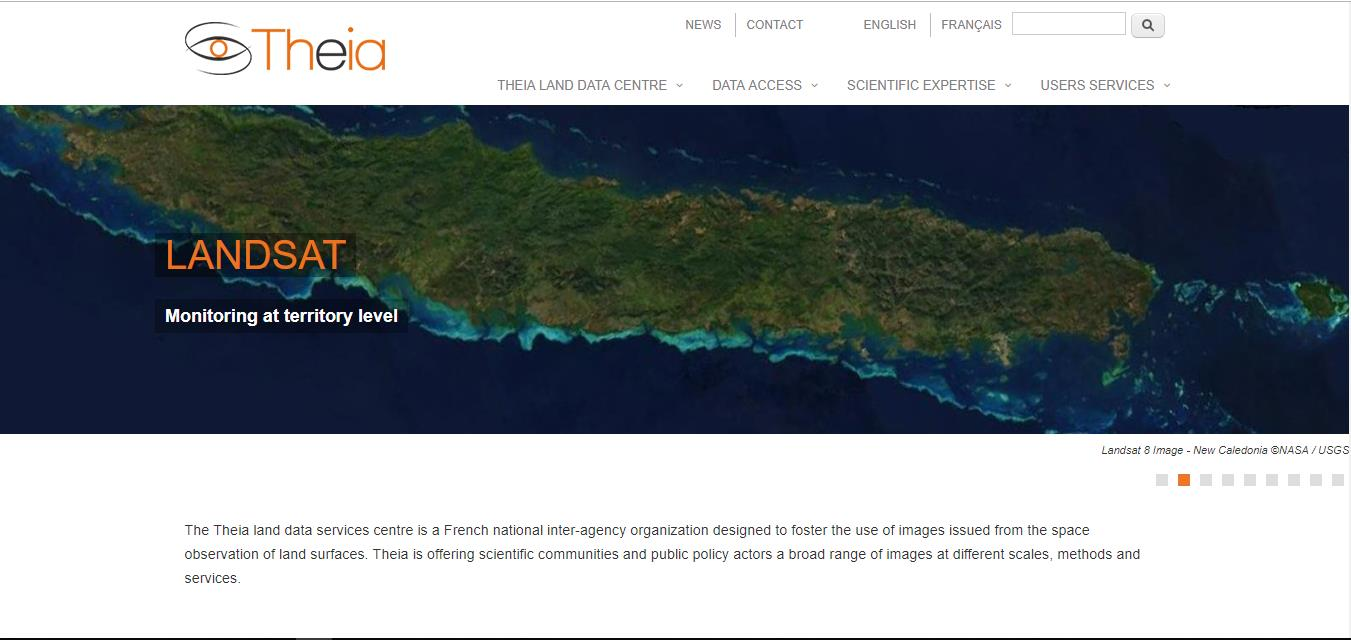
\includegraphics[width=0.5\textwidth]{pictures/Theia_Land_Data_Center}
\caption{Theia- Land Data Center}
\label{labelgambar7}
\end{figure}
\end{enumerate}


\chapter{WFS DAN WCS}
\section{WFS DAN WCS}

\subsection{Web Feature Service(WFS)}
Web Feature Service (WFS) merupakan penyedia antarmuka yang memungkinkan permintaan atau request untuk fitur geografis di seluruh web menggunakan panggilan platform-independen. operasi dasarnya termasuk GetCapabilities, DescribeFeatureType dan GetFeature. Seseorang dapat berpikir tentang fitur geografis sebagai "kode sumber" di belakang peta, sedangkan antarmuka WMS atau online pemetaan portal keramik seperti Google Maps kembali hanya gambar, yang akhir-pengguna tidak dapat mengedit atau spasial menganalisis \cite{franto2015integrasi}.
WFS dapat berupa layanan publikasi data geospasial pada tingkat fitur data spasial melalui media web. Disamping penyajian data spasial melalui gambar/image yang dilakukan oleh WMS, klien dapat memperoleh informasi data geospasial hingga ke lever fitur yaitu baik geometri maupun data atributnya. Spesifikasi OGC untuk WFS menggunakan teknologi XML (Extensible Markup Language) dan protokol HTTP (Hyper Text Transfer Protocol) sebagai media penyampaiannya \cite{ayuningtias2014aplikasi}.
Web Feature Service (WFS) merupakan suatu perubahan dalam pembuatan, pertukaran dan modifikasi data informasi geografis dalam internet. Perbedanya dengan WMS terletak pada kemampuan WFS melakukan publikasi data spasial hingga pada tingkatan unsur. Client WFS dapat memperoleh informasi unsur spasial dalam bentuk vektor, baik pada tingkatan geometri maupun atributnya. Salah satu format data WFS yang paling sering digunakan adalah GeoJSON. GeoJSON menurut situs resminya geojson.org adalah suatu format encoding dari berbagai struktur data spasial. GeoJSON mencakup format-format data geometry berikut: Point, LineString, Polygon, MultiPoint, MultiLineString, dan MultiPolygon \cite{wibowoseminar}.
Meskipun sumber data dalam layanan WFS bervariasi tergantung pada server yang digunakan, database geografis, shapefile adalah suatu keharusan. OGC tidak memberlakukan batasan apa pun pada masalah ini. Selain itu, data yang disajikan adalah GML \cite{putri2018pembuatan}, format pertukaran data berbasis XML. Selain itu, tergantung pada server yang digunakan dalam format berbeda seperti GeoJSON, CSV (Comma Seperated Value), KML, DXF, GeoRSS dapat dilayani.

Dengan WFS, tidak ada aliran data langsung dari server ke klien, sehingga data dapat ditransmisikan dari klien ke server. Pengguna dapat mengubah data pada data yang masuk (menyisipkan, memperbarui, menghapus) untuk mengirimkannya ke server dan memperbarui data. Layanan WFS tersebut disebut Transactional WFS atau WFS-T \cite{khair2016pembuatan}. Anda dapat menemukan beberapa server yang melayani WFS di bawah ini.
Feature server adalah,
\begin{enumerate}
\item GeoServer,
\item Server ArcGIS,
\item Server QGIS,
\item MapServer (TinyOWS)
\end{enumerate}

Desktop QGIS:
\begin{enumerate}
\item ArcGIS Desktop (Ekstensi Interoperabilitas),
\item uDig,
\item OpenLayers,
\item Gaia 3,
\item GRASS GIS
\end{enumerate}

Sebuah web mapping server yang dapat mengembalikan data geografis aktual yang terdiri dari gambar peta tersebut. Hal ini memungkinkan pengguna untuk dapat membuat peta mereka sendiri dan aplikasi dari data, untuk mengkonversi data antara format tertentu, dan dapat melakukan manipulasi data geografis baku dilayani. Protokol yang digunakan untuk mengembalikan suatu data fitur geografis disebut Web Fitur Layanan (WFS) \cite{purab2015penyajian}. Pada gambar \ref{labelgambar1} menunjukkan proses dimana WFS mengubah permintaan menjadi respons.

\begin{figure}[htbp]
\centering
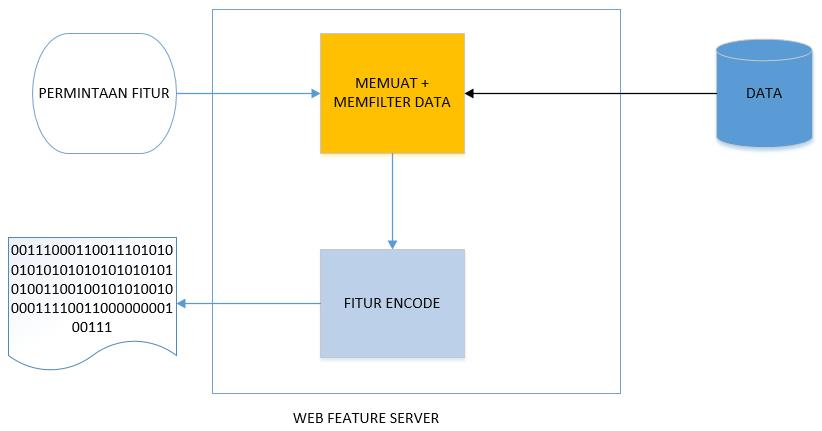
\includegraphics[width=1\textwidth]{pictures/WFS_RSPN}
\caption{menunjukkan bagaimana WFS mengubah permintaan menjadi respons}
\label{labelgambar1}
\end{figure}

\chapter{Datum WGS84 DAN NAD83}
\section{Datum WGS84 DAN NAD83}
\subsection{Pengertian DATUM}

Datum merupakan sebuah istilah yang dicetuskan oleh Alfred North Whitehead untuk menunjukan berbagai varian informasi yang dimiliki oleh entitas aktual. Di dalam sistem filsafat proses, datum dapat diperoleh melalui peristiwa konkresi. Setiap entitas aktual memiliki berbagai macam datum. Saat entitas aktual sudah mencapai kepenuhannya, satisfaction, ia akan mengalami peristiwa yang biasa disebut konkresi. Peristiwa inilah yang membuat entitas aktual memberikan informasi-informasi bagi potensi terbentuknya entitas aktual lainnya. Informasi-informasi inilah yang disebut dengan datum. Di dalam setiap peristiwa prehensi datum dapat diterima sebagai potensi informasi yang relevan dalam pembentukan entitas aktual dan datum dapat ditolak berdasarkan pertimbangan relevansi entitas aktual yang akan terbentuk. Proses diterimanya datum sebagai informasi relevan dari entitas aktual lainnya melalui peristiwa prehensi yang disebut sebagai prehensi positif. Proses ditolaknya datum sebagai informasi relevan dari entitas aktual lainnya melalui peristiwa prehensi yang disebut sebagai prehensi negatif.
Satu potensi entitas aktual merasakan banyak datum dari berbagai entitas aktual yang ada di dalam semesta. Ketika entitas aktual hendak mewujudkan dirinya, ia akan merasakan banyak datum. Datum yang dirasakan oleh entitas aktual merupakan datum-datum yang telah mengalami proses penolakan dan proses penerimaan yang panjang di dalam ruang dan waktu oleh entitas aktual melalui prehensi. Datum yang diterima sebagai informasi yang relevan bagi suatu potensi terbentuknya entitas aktual yang baru, merupakan datum yang telah mengalami proses ditolak dan diterima melalui prehensi oleh entitas aktual sebelumnya. Datum yang lahir dari peristiwa konkresi merupakan datum-datum yang khas dan baru. Datum yang satu berbeda dengan datum yang lainnya. Sebuah entitas aktual terdiri dari berbagai macam datum. Datum-datum ini terbentuk secara unik melalui peristiwa konkresi.
Datum geodetik atau referensi permukaan atau georeferensi merupakan parameter yang digunakan sebagai acuan untuk mendefinisikan geometri ellipsoid bumi. Datum geodetik diukur menggunakan metode manual hingga metode yang memiliki akurasi yang lebih akurat, yakni menggunakan satelit.

\begin{table}[h]
\caption{Ellipsoid Geosentrik WGS84}
\centering
\begin{tabular}{p{1.25in}p{1.25in}p{1.25in}}
\hline
Parameter&Notasi&Nilai\\
\hline
Sumbu Panjang & a & 6378137 m\\
Penggepengan & f & 1/298.257223563\\
Kecepatan Sudut Bumi & w & 7292115.0 x 10$^{-11}$ rad s$^{-1}$\\
Konstanta Gravitasi Bumi ( termasuk massa atmosfernya ) & GM & 3986004.418 x 108 m$^3$$ s^{-2}$\\
\hline
\end{tabular}
\label{table:contoh}
\end{table}





\bibliographystyle{IEEEtran} 
%\def\bibfont{\normalsize}
\bibliography{references}


%%%%%%%%%%%%%%%
%%  The default LaTeX Index
%%  Don't need to add any commands before \begin{document}
\printindex

%%%% Making an index
%% 
%% 1. Make index entries, don't leave any spaces so that they
%% will be sorted correctly.
%% 
%% \index{term}
%% \index{term!subterm}
%% \index{term!subterm!subsubterm}
%% 
%% 2. Run LaTeX several times to produce <filename>.idx
%% 
%% 3. On command line, type  makeindx <filename> which
%% will produce <filename>.ind 
%% 
%% 4. Type \printindex to make the index appear in your book.
%% 
%% 5. If you would like to edit <filename>.ind 
%% you may do so. See docs.pdf for more information.
%% 
%%%%%%%%%%%%%%%%%%%%%%%%%%%%%%

%%%%%%%%%%%%%% Making Multiple Indices %%%%%%%%%%%%%%%%
%% 1. 
%% \usepackage{multind}
%% \makeindex{book}
%% \makeindex{authors}
%% \begin{document}
%% 
%% 2.
%% % add index terms to your book, ie,
%% \index{book}{A term to go to the topic index}
%% \index{authors}{Put this author in the author index}
%% 
%% \index{book}{Cows}
%% \index{book}{Cows!Jersey}
%% \index{book}{Cows!Jersey!Brown}
%% 
%% \index{author}{Douglas Adams}
%% \index{author}{Boethius}
%% \index{author}{Mark Twain}
%% 
%% 3. On command line type 
%% makeindex topic 
%% makeindex authors
%% 
%% 4.
%% this is a Wiley command to make the indices print:
%% \multiprintindex{book}{Topic index}
%% \multiprintindex{authors}{Author index}

\end{document}

